% This is file JFM2esam.tex
% first release v1.0, 20th October 1996
%       release v1.01, 29th October 1996
%       release v1.1, 25th June 1997
%       release v2.0, 27th July 2004
%       release v3.0, 16th July 2014
%   (based on JFMsampl.tex v1.3 for LaTeX2.09)
% Copyright (C) 1996, 1997, 2014 Cambridge University Press

\documentclass{jfm}
\usepackage{graphicx}
%\usepackage{epstopdf, epsfig}
\usepackage{physics}
\usepackage{subfig}
\usepackage{minted}
\usepackage{enumitem,amssymb}
\newlist{todolist}{itemize}{2}
\setlist[todolist]{label=$\square$}
\usepackage{pifont}
\newcommand{\cmark}{\ding{51}}%
\newcommand{\xmark}{\ding{55}}%
\newcommand{\done}{\rlap{$\square$}{\raisebox{2pt}{\large\hspace{1pt}\cmark}}%
\hspace{-2.5pt}}
\newcommand{\wontfix}{\rlap{$\square$}{\large\hspace{1pt}\xmark}}

\newtheorem{lemma}{Lemma}
\newtheorem{corollary}{Corollary}

\newcommand{\cz}{c_{\zeta}}
\newcommand{\cs}{c_{\psi}}
\newcommand{\ct}{c_{\theta}}
\newcommand{\csz}{c_{\psi \zeta}}
\newcommand{\czs}{c_{\zeta \psi}}
\newcommand{\czz}{c_{\zeta \zeta}}
\newcommand{\ctz}{c_{\theta \zeta}}
\newcommand{\czt}{c_{\zeta \theta}}
\newcommand{\cst}{c_{\psi \theta}}
\newcommand{\cts}{c_{\theta \psi}}
\newcommand{\Ray}{\mbox{\textit{Ra}}}  % Rayleigh number


% \shorttitle{CE2 Busse Annulus}
% \shortauthor{J. S. Oishi, S. M. Tobias, K. J. Burns, J. B. Marston}

\title{Busse Annulus CE2 Crashing Notes}

% \author{Jeffrey S. Oishi\aff{1}
%   \corresp{\email{joishi@bates.edu}},
%   Steven M. Tobias\aff{2},
%   Keaton J. Burns\aff{3
% }
%  \and J. B. Marston\aff{4}}

% \affiliation{\aff{1}Department of Physics \& Astronomy, Bates College,
% Lewiston, ME 04240, USA
% \aff{2}Department of Applied Mathematics, University of
% Leeds, Leeds LS2 9JT, UK
% \aff{3}Center for Computational Astrophysics, Flatiron Institute, New York, NY 10010, USA
% \aff{4}Department of Physics, Brown University, Providence, RI 02912, USA
% }

\begin{document}

\maketitle

\begin{abstract}
  The CE2 Busse Annulus runs crash when $\Ray$ is above a certain value.
At lower driving, it correctly reproduces QL results; when biased to have the correct 2-jet solution, it \emph{also} reproduces the DNS results.
This is a mystery; here I write up progress to this point and some questions to ponder for next week's meeting.
\end{abstract}

\begin{keywords}
\end{keywords}

\section{The Problem}
\label{sec:intro}

I've been trying three fiducial runs, in table~\ref{tab:runs}.
The parameters are identical to similarly named runs in our 2018 GQL paper.
%
\begin{table}
  \begin{center}
\def~{\hphantom{0}}
  \begin{tabular}{lccc}
      Run  & $\Rey$ & $C$ & $\beta$ \\[3pt]
       A  & 76000   & 0. & 2800\\
       B  & $10^8$  & 0.316 & $7.07\times10^5$\\
       C  & $8\times10^7$ & 0 & $5\times10^5$\\
  \end{tabular}
  \caption{Runs}
  \label{tab:runs}
  \end{center}
\end{table}
%
Run A works just fine; it shows the same results as a QL simulation.
\begin{figure}
  \centering
  
  \subfloat{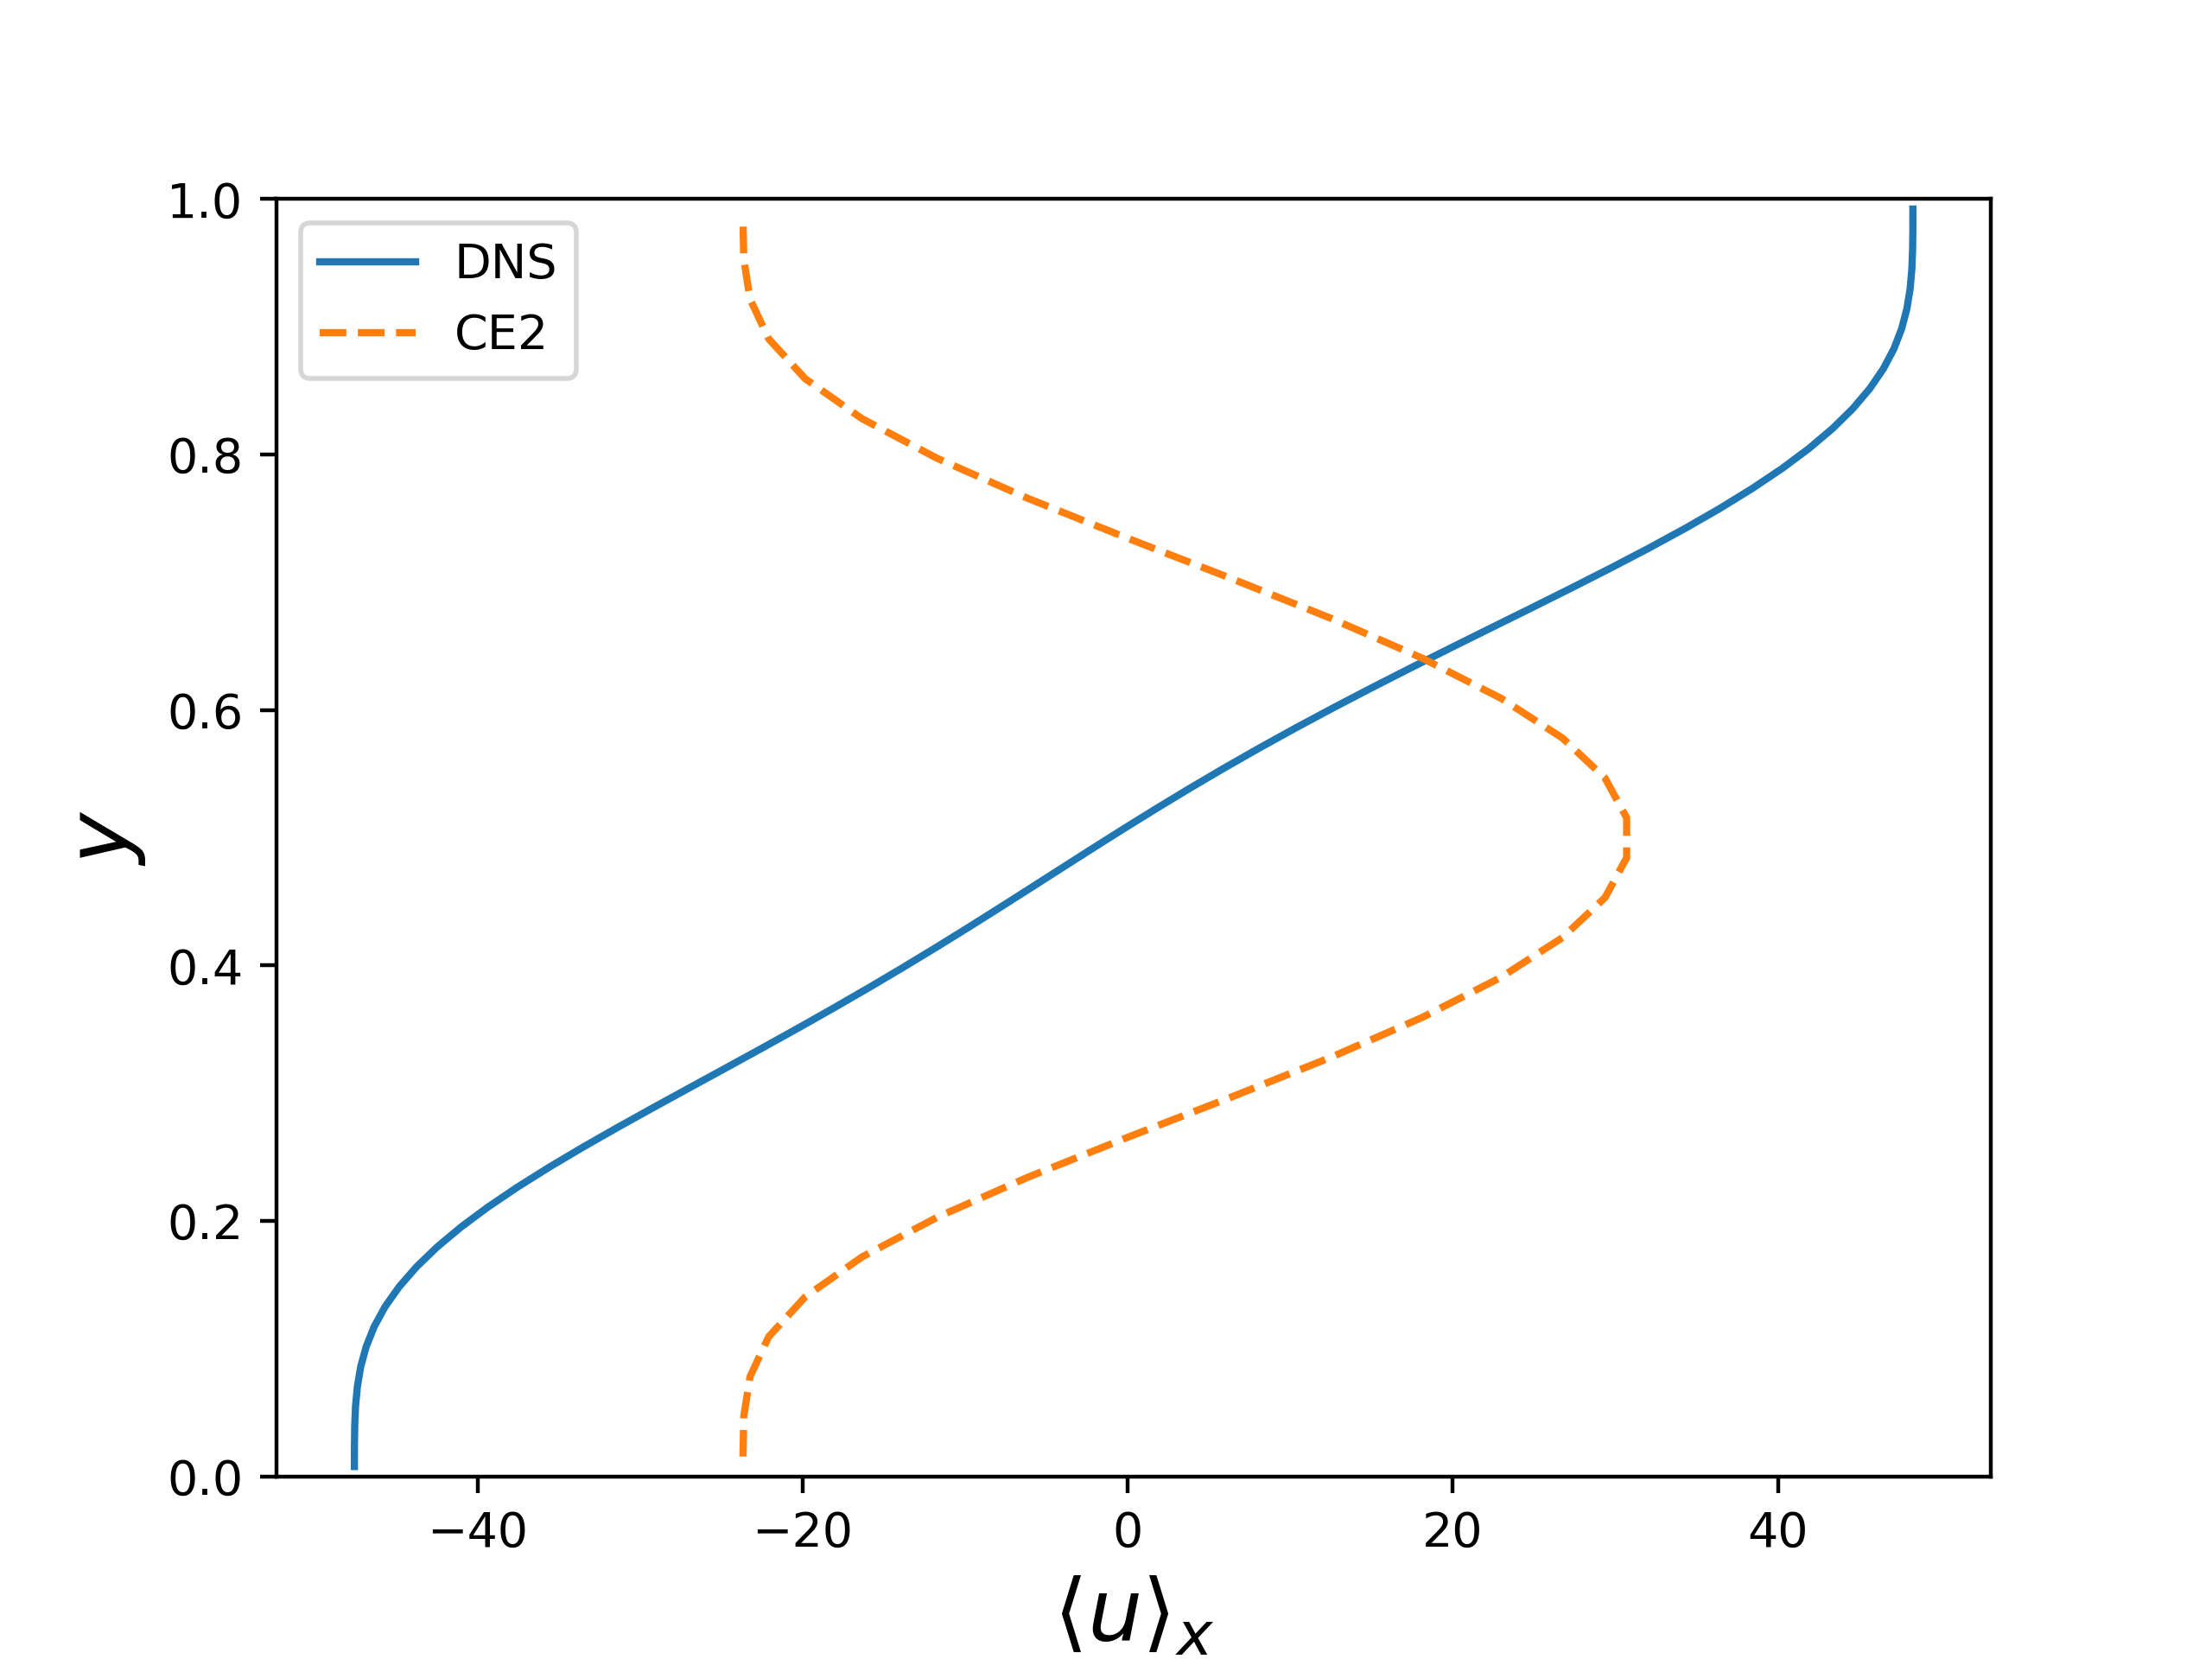
\includegraphics[width=0.5\textwidth]{umean_dns_ce2_run_A.png}}
  \hfill
  \subfloat{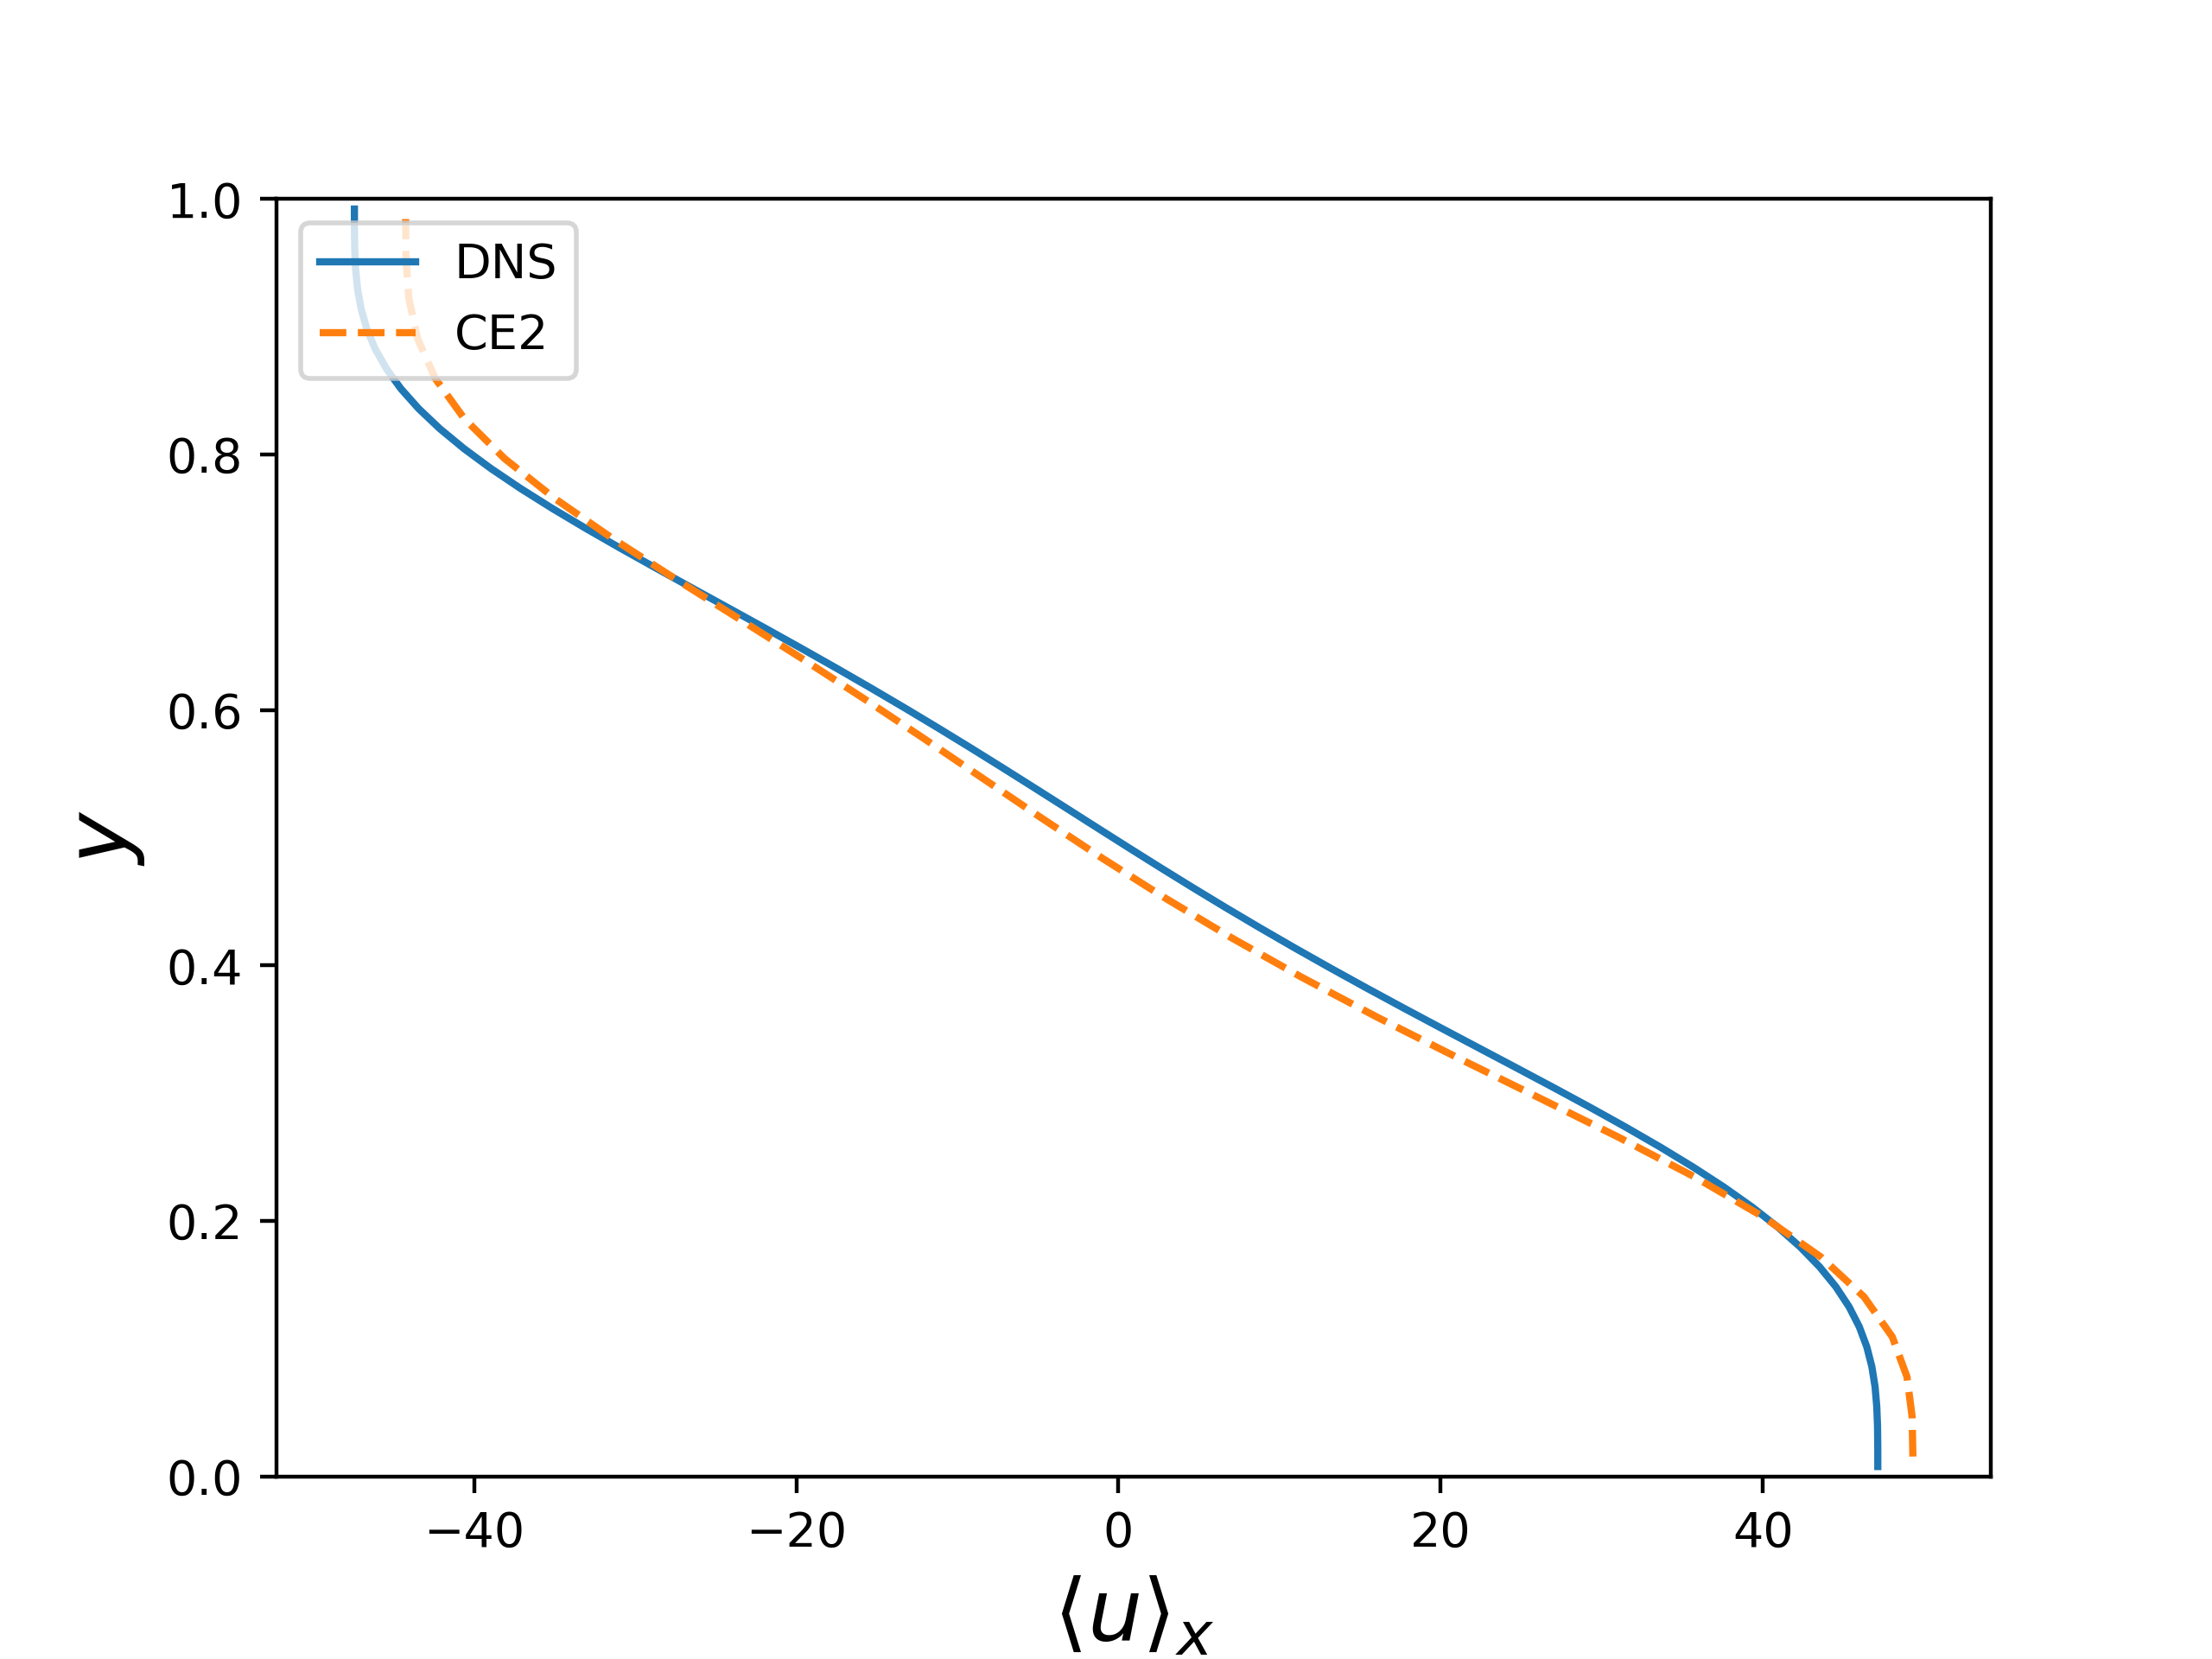
\includegraphics[width=0.5\textwidth]{umean_dns_ce2_run_I.png}}
  \caption{Comparison of mean flow between (left) run A and DNS (right) a CE2 run initialized with a large-amplitude 2-jet profile and DNS. Note that on the left, the CE2 calculation is very close to the QL results from our 2018 paper. On the right, the CE2 and DNS solutions are very similar.}
  \label{fig:mean_comparison}
\end{figure}
If we bias it by starting from a 2-jet solution with an amplitude selected to match the DNS, it will continue that solution in time (see figure~\ref{fig:mean_comparison}.

However, run B crashes after a few hundred timesteps with $dt = 2.5\times 10^{-5}$; lowering the timestep by a factor of ten buys about ten times more timesteps:
this is not a timestepping problem.
A slightly more quantitative way of looking at this is to calculate the exponential growth rate, $\left<c_\psi\right> \propto e^{\gamma t}$.
For $dt = 2.5\times 10^{-6}$, $\gamma = 8655$; at $dt = 6.25\times 10^{-7}$, $\gamma = 8429$.
This is a $\sim 3 \%$ change in growth rate for a factor of 4 increase in timestep.



\section{Growing means}
\label{sec:means}

One thing that became apparent is that the mean over the \emph{entire volume}, 
\begin{equation}
  \label{eq:mean}
  \left< Q\right> = \frac{\int Q dV}{V},
\end{equation}
of the first cumulants $c_\theta$, $c_\psi$, and $c_\zeta$ were growing exponentially with time in all runs.
Because of the use of sin/cos basis functions, it turns out that what I had been doing to prevent growth of the mean wasn't working.
This is because setting the zero mode of a \emph{Fourier} series will kill the mean, and the same is true for cosines, for \emph{sine} series, the mean is distributed over all odd modes.
There is no simple prescription any more for projecting the mean to zero, so I instead simply subtract the mean on the grid from the first cumulants.
This works for run A, as seen in figure~\ref{fig:run_A_mean}, even if we only subtract the mean from $c_\theta$. 
Frustratingly, for run B, this does \emph{not} work (figure~\ref{fig:run_B_mean}), even if we subtract means from \emph{all} first cumulants.
In both runs, the mean is being subtracted at every timestep.
%
\begin{figure}
  \centering
  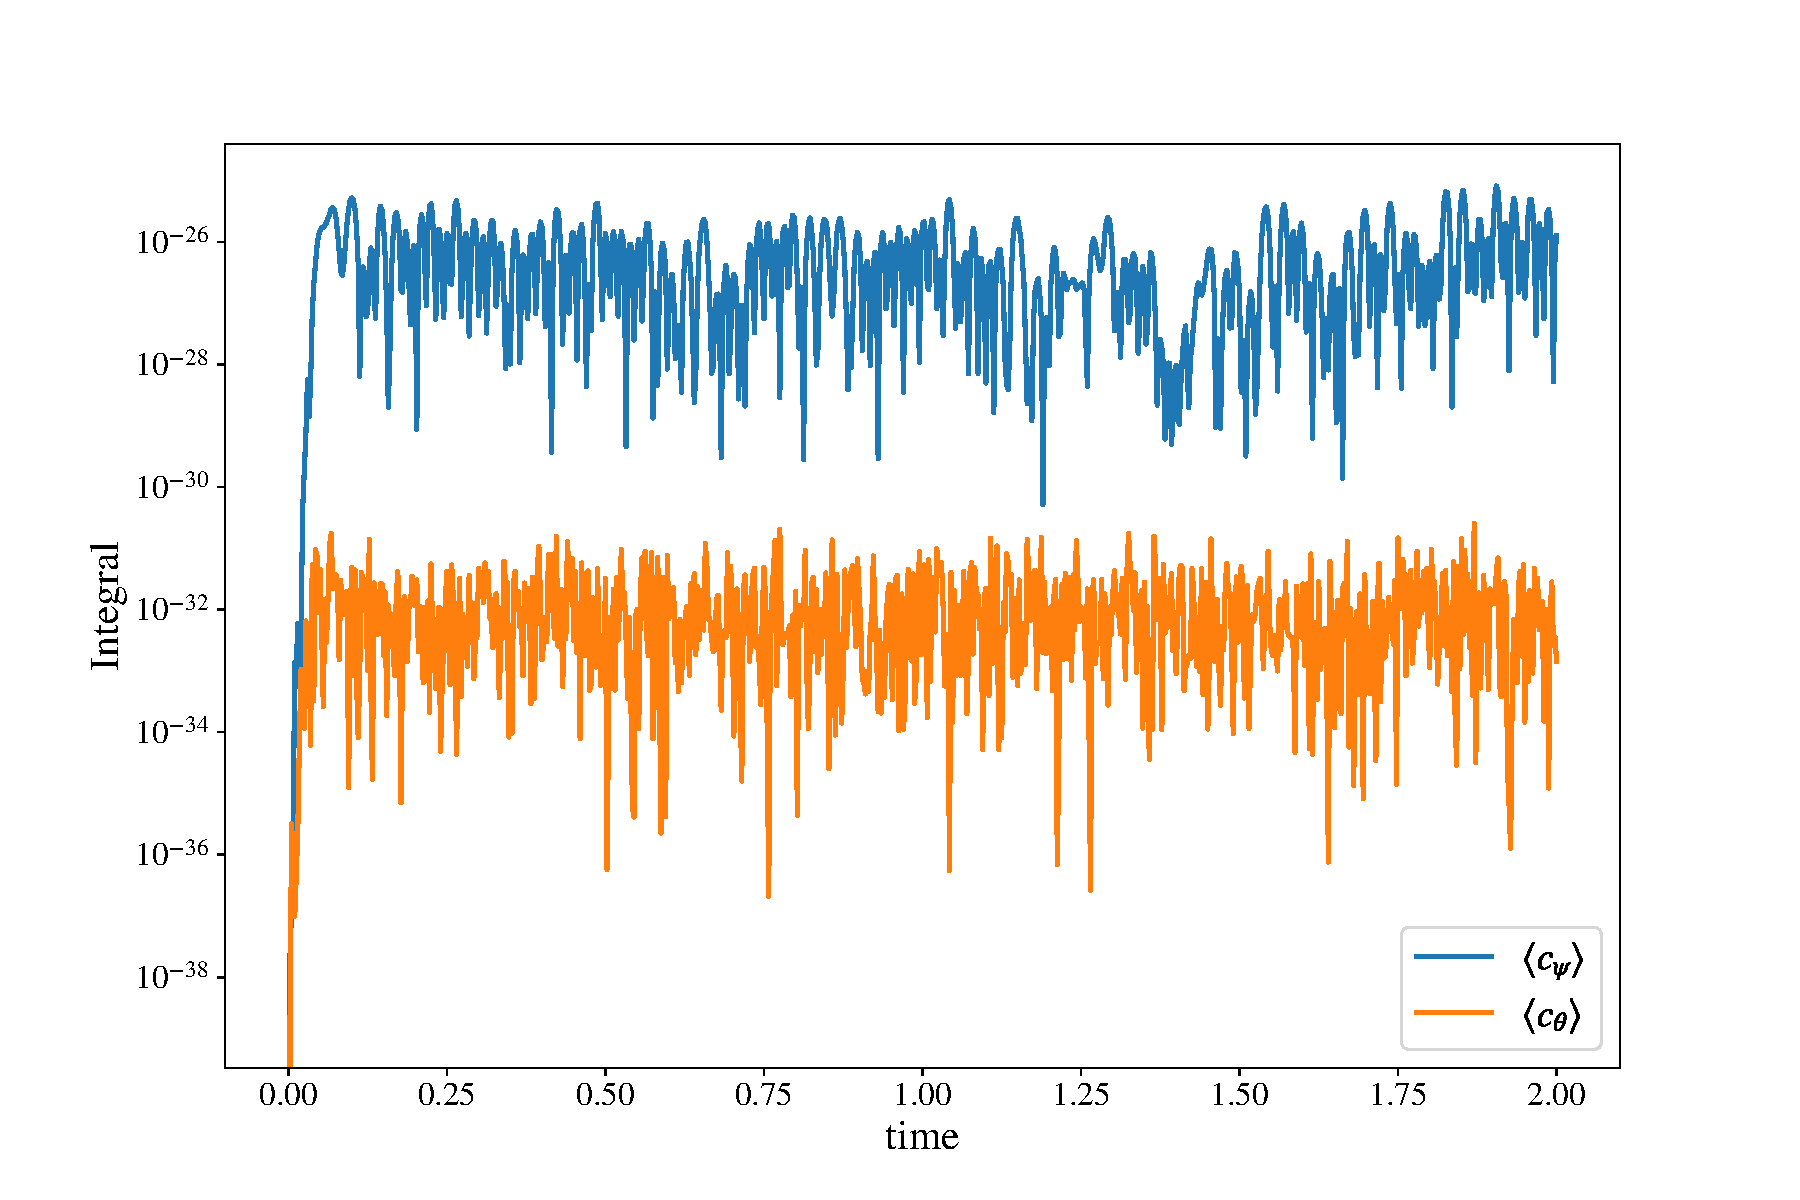
\includegraphics[width=\textwidth]{run_A_integrals.pdf}
  \caption{Mean first cumulants for run A. Note that they do not grow exponentially in time.}
    \label{fig:run_A_mean}
\end{figure}
%
\begin{figure}
  \centering
  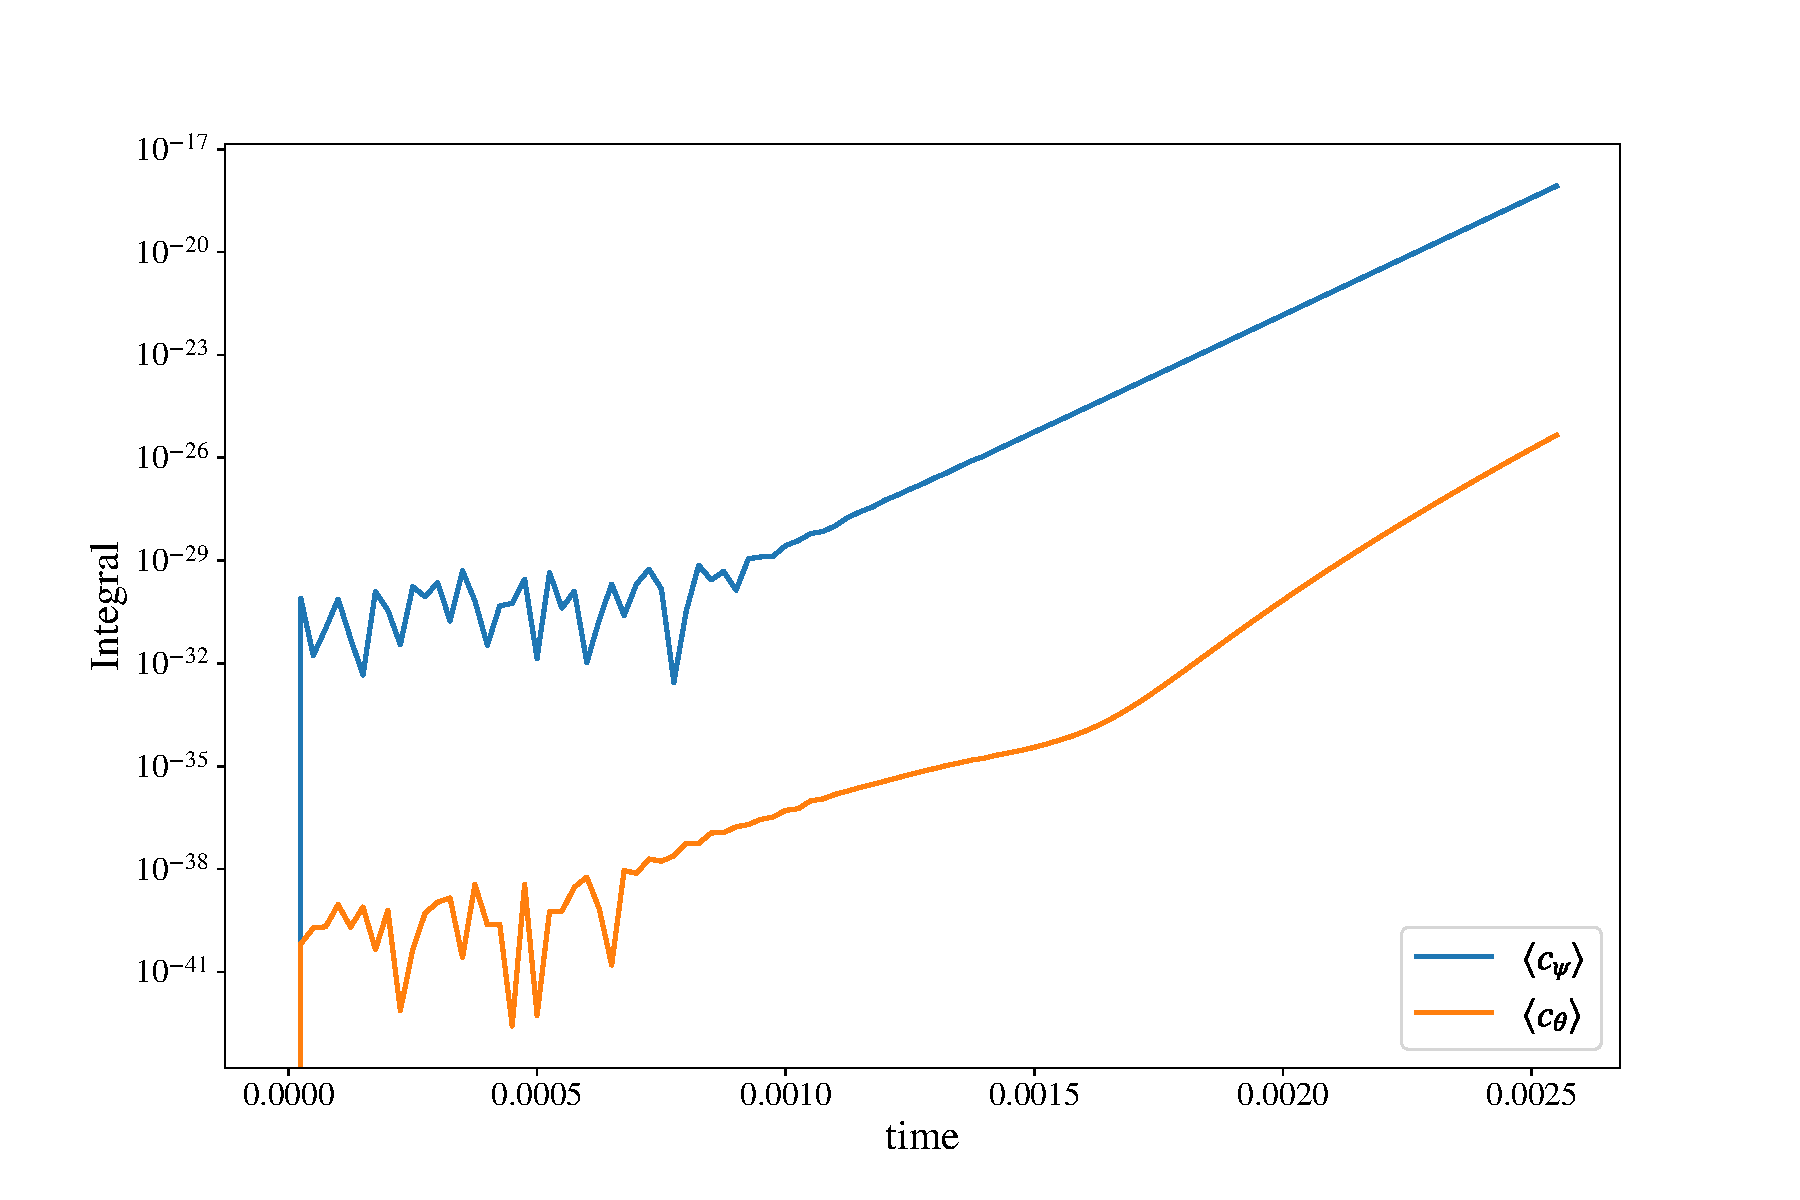
\includegraphics[width=\textwidth]{run_B_integrals.pdf}
  \caption{Mean first cumulants for run B. They still show exponential growth.}
  \label{fig:run_B_mean}
\end{figure}

\section{Removing negative eigenvalues}
\label{sec:eigenvalues}

Kraichnan (1980) (equation 4) states that a necessary and sufficient criterion to ensure the PDF is nowhere negative is that the ensemble average of the square of every real polynomial of a given random variable $x$ be non-negative,
\begin{equation}
  \label{eq:Kraichnan_4}
  % \left{\left(\sum_{r = 0}^{n}\lambda_r x^r\right)\right} = \sum_{r,s = 0}^{n} \lambda_s \lambda_r  \geq 0
  \left\{\left(\sum_{r = 0}^{n}\lambda_r x^r\right)^2\right\} = \sum_{r,s = 0}^{n} \lambda_s \lambda_r \left\{x^{r+s} \right\} \geq 0
\end{equation}
This is equivalent to saying that the symmetric matrix $\{ x^{r+s}\}$ has no negative eigenvalues.

While I can clearly see how this is necessary, I don't see how it is sufficient; this argument invokes Carlemon's criterion which I haven't investigated.

In our case, this turns into the criteria that the second cumulants have no negative eigenvalues.
To calculate this, I take the second cumulants $\hat{c}_{\theta \theta}(k_x, k_{y1}, k_{y2})$ (for example) in spectral space, and for each $k_x$ I define a square matrix $A_{ij} = \hat{c}_{\theta \theta}(k_x, i, j)$.
I then find its Hermitian part $\mathsf{H} = (\mathsf{A} + \mathsf{A}^\dagger)/2$ and find the eigenvalues $\lambda_i$ and eigenvectors $\mathbf{q_i}$ of $H$.
For each $\lambda_i < -\epsilon$ where $\epsilon = 10^{-12}$ by default (though I typically use $10^{-8}$ or larger), I set that $\lambda_i = 0$.
Finally, I construct a diagonal matrix $\mathsf{\Lambda}$ of the corrected eigenvalues and a matrix $\mathsf{Q}$ of the eigenvectors, and reconstruct $\mathsf{A}' = \mathsf{Q} \mathsf{\Lambda} \mathsf{Q}^{-1}$.
Happily, since $\mathsf{H}$ is normal, $\mathsf{Q}$ is unitary, and we don't even need to invert it.


\subsection{Eigenvalue projection code}
\label{sec:eig_code}
Below is the code that does the projection.
The important part is the \texttt{project} method.


\begin{minted}[fontsize=\tiny]{python}
import scipy.linalg as linalg
import numpy as np

import logging
logger = logging.getLogger(__name__)

class EigenvalueProjection:
    def __init__(self, domain):
        self.domain = domain
        self._build_subcommunicator()

        dtype = 'complex128'
        self.recbuf = None
        self.workbuf = None
        if self.rank == 0:
            self.local_shape = self.domain.local_coeff_shape
            self.global_shape = self.domain.global_coeff_shape
            self.rec_shape = [self.size,] + list(self.local_shape)
            self.work_shape = [self.local_shape[0],] + list(self.global_shape[1:3])
            self.recbuf = np.empty(self.rec_shape, dtype=dtype)
            self.workbuf = np.empty(self.work_shape, dtype=dtype)
            logger.debug("dtype = {}".format(self.recbuf.dtype))
            logger.debug("local_shape = {}".format(self.local_shape))
            logger.debug("rec_shape = {}".format(self.rec_shape))
            logger.debug("work_shape = {}".format(self.work_shape))

    def _build_subcommunicator(self):
        if self.domain.dist.comm_cart.size == 1:
            self.comm = self.domain.dist.comm_cart
        else:
            self.comm = self.domain.dist.comm_cart.Sub([False,True])
        self.rank = self.comm.rank
        self.size = self.comm.size

    def project(self, data, thresh=1e-12):
        self.gather(data)
        # do the projection
        # A = Q Lambda Qinv
        # where Lambda is the matrix of eigenvalues and Q is the matrix of eigenvectors,
        # and we delete all negative eigenvalues from Lambda
        if self.rank == 0:
            nx = self.local_shape[0]
            for m in range(nx):
                A = self.workbuf[m,:,:]
                H = 0.5*(A + A.conj().T) # hermitian part
                AH = A - H # antihermitian part
                # A is a positive definite matrix iff H, the hermitian part, is positive definite
                evals, Q = linalg.eigh(H)
                index = (evals < -thresh) # find negative eigenvalues
                if np.any(index):
                    logger.warning("{} negative eigenvalues found for {} at x-mode {}".format(np.sum(index),data.name,m))
                evals[index] = 0
                Qinv = Q.conj().T # if input is Normal, Q is unitary, and all H matricies are Normal!
                Lambda = np.diag(evals)
                self.workbuf[m,:,:] = Q @ (Lambda @ Qinv) + AH
        self.scatter(data)

    def gather(self, data):
        self.comm.Gather(data['c'], self.recbuf, root=0)
        if self.rank == 0:
            blocksize = self.rec_shape[2]
            for block in range(self.rec_shape[0]):
                self.workbuf[:,block*blocksize:(block+1)*blocksize,:] = self.recbuf[block]

    def scatter(self, data):
        if self.rank == 0:
            blocksize = self.rec_shape[2]
            for block in range(self.rec_shape[0]):
                self.recbuf[block] = self.workbuf[:,block*blocksize:(block+1)*blocksize,:]
        self.comm.Scatter(self.recbuf,data['c'], root=0)

\end{minted}


\section{Model Equations}
\label{sec:model-eqations}

We consider the equations for the Busse annulus.
We write the equation of motion in terms of the $z$-component of the vorticity, $\zeta$.

\begin{equation}
  \label{eq:zeta_eom}
  \pdv{\zeta}{t} + J(\psi, \zeta) - \beta \pdv{\psi}{x} = -\frac{\Ray}{\Pran} \pdv{\theta}{x} -C |\beta|^{1/2} \zeta + \laplacian{\zeta}
\end{equation}
The streamfunction $\psi$ is defined by
\begin{equation}
  \label{eq:zeta_def}
  \zeta = \laplacian{\psi},
\end{equation}
which means the $x$ velocity $u = -\pdv*{\psi}{y}$ and the $y$ velocity $v = \pdv*{\psi}{x}$. $J(A, B) = \pdv*{A}{x}\pdv*{B}{y} - \pdv*{A}{y}\pdv*{B}{x}$ is the Jacobian. 
The perturbed temperature is given by $\theta$, which obeys the dynamical equation
%
\begin{equation}
  \label{eq:theta}
  \pdv{\theta}{t} + J(\psi, \theta) = -\pdv{\psi}{x} + \frac{1}{\Pran} \nabla^2 \theta.
\end{equation}
The system is thus governed by four dimensionless parameters, $\beta$, $C$, $\Pran = \nu/
\kappa$, and $\Ray = \alpha g \Delta T d^3/\nu \kappa$

For the CE2 expansion, we need equations for the first cumulants $\cz$ and $\ct$, and the second cumulants $\czs$, $\czz$, $\ctz$, and $\czt$. 
While second cumulants involving $\psi$ and $\zeta$ are related by the gradient operators, e.g. $\czz = \nabla_2^2 \czs$, those involving $\theta$ require use of the symmetry $\ctz(y_1, y_2, \xi) = \czt(y_2, y_1, -\xi)$.

We solve dynamical equations for $\cz$,
\begin{equation}
  \label{eq:cz}
  \pdv{\cz}{t} = - \qty(\pdv{y_1} + \pdv{y_2}) \pdv{\csz}{\xi}\eval_{\xi \to 0}^{y_1 \to y_2} - C |\beta|^{1/2} \cz + \pdv[2]{\cz}{y_1},
\end{equation}

\begin{equation}
  \label{eq:czz}
  \begin{split}
    \pdv{\czz}{t} &= \pdv{\cs}{y_1} \pdv{\czz}{\xi} - \qty(\pdv{\cz}{y_1} - \beta) \pdv{\csz}{\xi} - \pdv{\cs}{y_2} \pdv{\czz}{\xi}  + \qty(\pdv{\cz}{y_2} - \beta) \pdv{\czs}{\xi}\\
    &+ \frac{\Ray}{\Pran} \qty(\pdv{\czt}{\xi} -  \pdv{\ctz}{\xi}) - 2C |\beta|^{1/2} \czz + (\nabla_1^2 + \nabla_2^2) \czz    
  \end{split}
\end{equation}

The first cumulant for $\theta$ evolves according to
\begin{equation}
  \label{eq:ct}
  \pdv{\ct}{t} = - \qty(\pdv{y_1} + \pdv{y_2}) \pdv{\cst}{\xi} \eval_{\xi \to 0}^{y_1 \to y_2} + \frac{1}{\Pran} \pdv[2]{\ct}{y_1}.
\end{equation}
For the second cumulant in $\theta$, we evolve $\ctz$,
\begin{equation}
  \label{eq:ctz}
  \begin{split}
    \pdv{\ctz}{t} &= \qty(\pdv{\cs}{y_1} - \pdv{\cs}{y_2}) \pdv{\ctz}{\xi} - \qty(1 + \pdv{\ct}{y_1}) \pdv{\csz}{\xi} + \qty(\pdv{\cz}{y_2} - \beta) \pdv{\cts}{\xi}\\
    &  - C |\beta|^{1/2} \ctz + \frac{1}{\Pran}\qty(\nabla_1^2 + \nabla_2^2) \ctz + \cdots,    
  \end{split}
\end{equation}
where $\cdots$ indicates the terms needed to ensure symmetry under exchange of $x_1, y_1$ and $x_2, y_2$.

\subsection{Parity}
\label{sec:parity}

We solve the system subject to impenetrable, stress-free boundary conditions in the $y$ dimension; it is periodic in $x$. 
This means that $\theta$, $\zeta$, and $\psi$ all have odd parity.
The action of the zonal average preserves the parity, and so we discretize the first cumulants $\cz$, $\ct$ using a $\sin$ series. 

% \bibliographystyle{jfm}
% % Note the spaces between the initials
% \bibliography{busse}

\end{document}

%  LocalWords:  DNS cumulants cumulant annulus Busse QL fiducial GQL
%  LocalWords:  lccc timesteps dt timestep timestepping dV Kraichnan
%  LocalWords:  Carlemon's ij Hermitian eigenvectors vorticity
%  LocalWords:  streamfunction Jacobian discretize
